% Created 2024-07-08 Mon 22:16
% Intended LaTeX compiler: pdflatex
\documentclass[11pt]{article}
\usepackage[utf8]{inputenc}
\usepackage[T1]{fontenc}
\usepackage{ragged2e}
\usepackage{caladea}
\usepackage{graphicx}
\usepackage{longtable}
\usepackage{wrapfig}
\usepackage{rotating}
\usepackage[normalem]{ulem}
\usepackage{amsmath}
\usepackage{amssymb}
\usepackage{capt-of}
\usepackage{hyperref}
\usepackage{fancyhdr}


\title{
 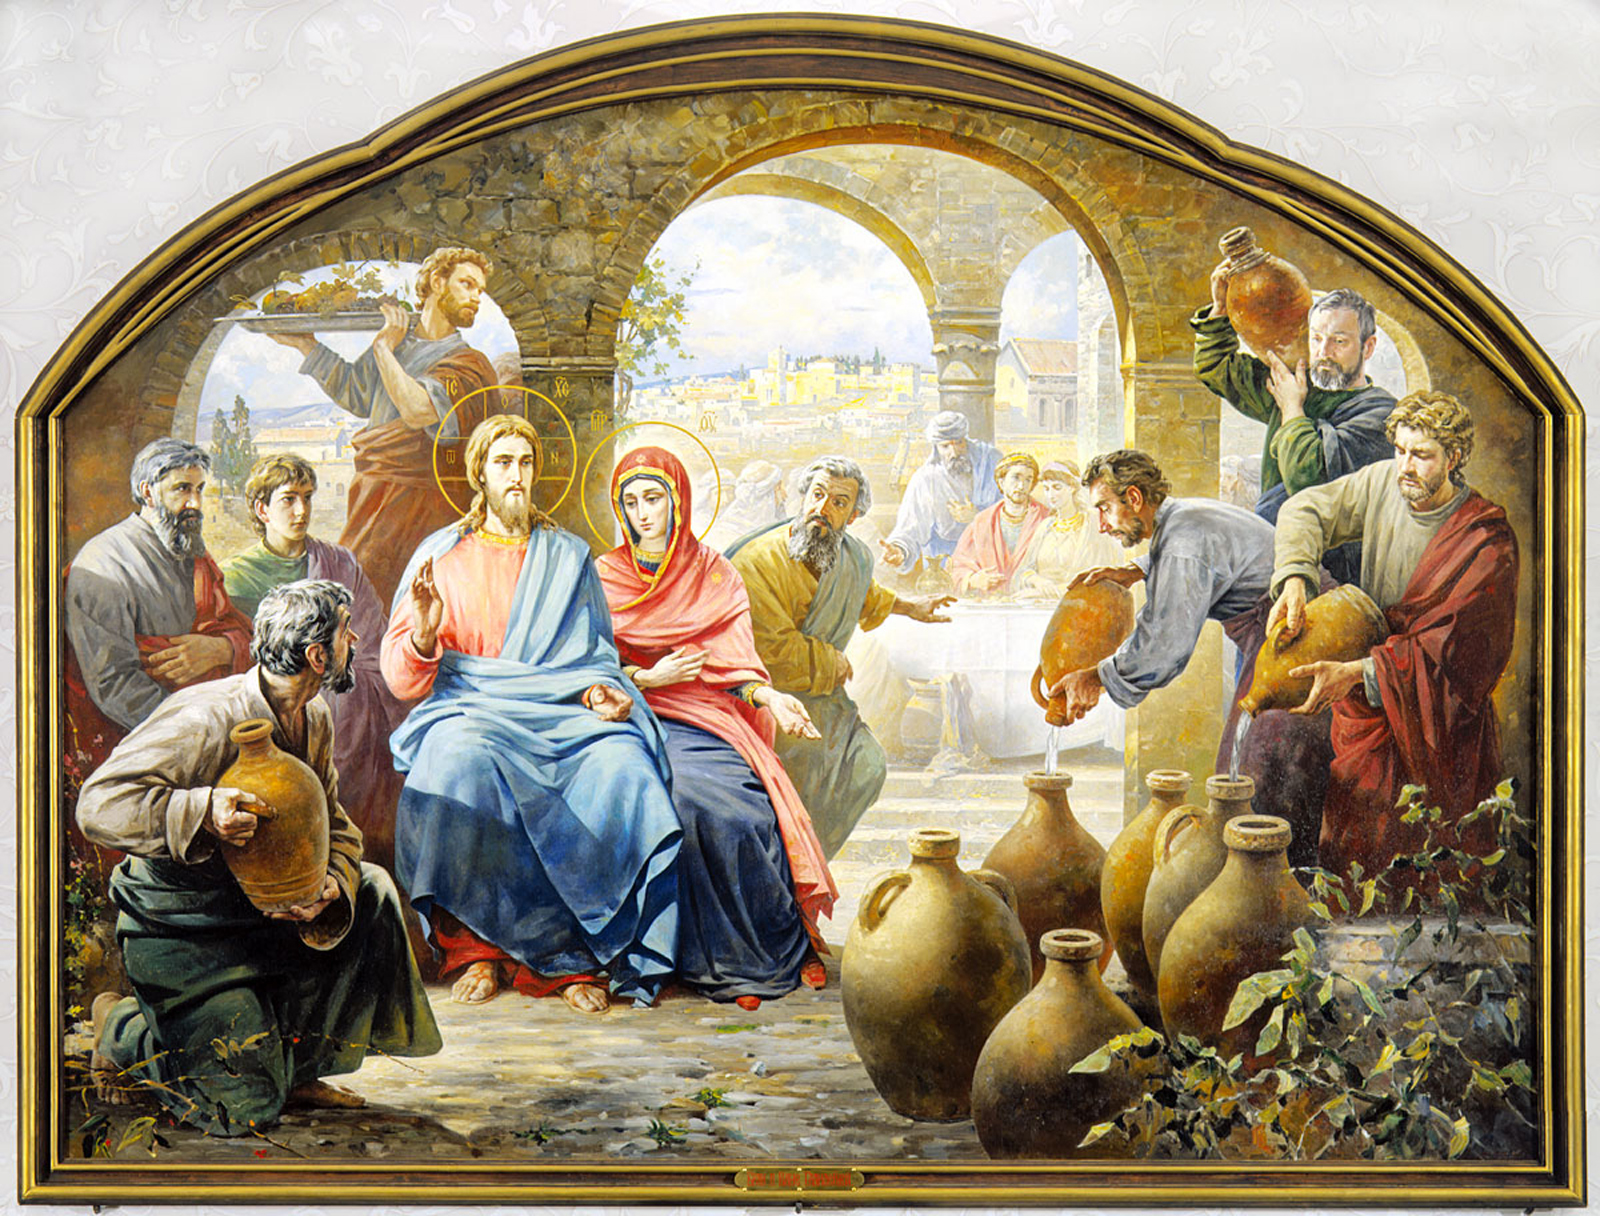
\includegraphics[trim={0 0 0 5cm} , scale=0.22]{./assets/imagem.jpg} \par
  NOVENA À NOSSA SENHORA DE CANÁ
}
\author{Garamog, Nina Freitas}
\date{Início da Novena: 28/12 - Data Litúrgica: 06/01 }

\addtolength{\topmargin}{-1.59999pt}

\begin{document}

\maketitle
\thispagestyle{empty} % Remove page number from the first page
\pagestyle{fancy}
\centering

% configuração do sumário
\renewcommand{\contentsname}{Sumário}

\newpage

\tableofcontents

\centering
\vfill
Visite-nos no Telegram: \url{https://t.me/CotidieNovena}
\newpage

\newpage

\section{Orações}
\subsection{Oração Inicial}

Oração Inicial para todos os dias

Ó Mãe das Bodas de Caná que alegria e paz ao saber que

todas as minhas necessidades estão em suas mãos.

Obrigado Mãe por se preocupar comigo. Mãe enche as

minhas talhas de expectativa de milagres que Seu Filho

vai operar em meus pedidos. Por isso recorro a Vós ó

Mãe, pois bem sei que Teu Filho sempre lhe escuta. Mãe,

se ainda não é o momento, \textbf{(apresenta a intenção da novena)} antecipa para mim esta hora.

\textbf{Pai-Nosso, Ave-Maria, Glória}

\subsection{Primeiro Dia}
\subsubsection*{Celebravam-se bodas em Caná.}
Nesse primeiro dia Maria quer que nossas vidas sejam sempre celebradas, como nas Bodas em Caná.

 Mãe venho pedir perdão a Deus por tantas vezes tê-Lo ofendido por não termos celebrado minha vida e por ter achado que ela era ruim, sem graça, não de acordo como queria. Muitas vezes a destruí vivendo a insatisfação e o descontentamento. Ó Mãe das Bodas de Caná ensina-me a aceitar a vida que Deus me deu e, com o que tenho e com quem for, sempre, sempre celebrar, pois a vida é dom de Deus. Mãe que eu aprenda a agradecer a cada manhã a minha vida, pois ela é uma festa; um presente de Deus.

Oração: Apresente sua vida, sua memória, sua mente e tudo que a envolve.  Conforme for apresentando peça à Maria para ir visitando assim como visitou Isabel, levando o Espírito Santo e enchendo sua vida de Amor e contentamento. Agradeça a Deus por esse momento. Obrigado ó Mãe das Bodas de Caná

Obrigado ó Mãe das Bodas de Caná. Obrigado Mãe, pois sei que sempre estás atenta as minhas necessidades. Ave Maria...

\subsection{Segundo dia}
\subsubsection*{ Achava-se ali a mãe de Jesus.}

Nesse segundo dia Jesus quer que aprendamos a agradecer a Deus por nos ter dado uma Mãe. Ao mesmo tempo que se agradece é vital reconhecer que é um momento de profunda cura para tantas pessoas que procuram suas mães e não a acham e outros que cansaram de procurar e nunca encontraram. Mãe, quantas pessoas sofrem as consequências de não terem o amor materno. Quantas consequências, como a carência, dificuldades no relacionamento, dificuldades em ser mãe. Que nesse momento possam saber que onde faltou a mãe terrena, a senhora se faz presente. Aqueles que procuram pelo amor de mãe podem procurar em Maria que acham. Maria vem suprir toda carência do amor materno, pois se faz presente.

Oração:  Deixe Maria te gerar de novo. Introduza Maria onde faltou a presença de sua mãe. Coloque os traços de Maria em sua mãe. Se não teve ou não conheceu, adote Maria como sua mãe. Se sinta amado (a) e dê o perdão à sua mãe. Agradeça Deus por esse momento. Obrigado ó Mãe das Bodas de Caná

\subsection{Terceiro Dia}
\subsubsection*{Como viesse a faltar vinho}
Nesse terceiro dia queremos aprender a conviver com as contrariedades da vida, com aquelas notícias que nos pegam de surpresa. Quantas coisas acabam em nossas vidas, como “que do nada”, quantas surpresas contrárias que não gostaríamos de ter. Nossa Mãe vem nesse dia a nos ensinar a sermos equilibrados, a sabermos lidar com as surpresas da vida, a não entrarmos em desespero, pois Ela está atenta a tudo.

Oração: Apresente toda a sua dificuldade em saber lidar com contrariedades, com as humilhações.  Coloque todo seu perfeccionismo, todo o controle que tem de tudo. Coloque sua dificuldade em lidar com as perdas. Vá pedindo a graça de conviver com as surpresas.  Apresente as notícias ruins que não gostaria de receber.  Apresente o que não gostaria de perder. Apresente as humilhações que não gostaria de passar. Deixe Maria lhe ensinar a viver nesse mundo cheio de contrariedades e surpresas. Agradeça a Deus por esse momento. Obrigado ó Mãe das Bodas de Caná

\subsection{Quarto Dia}
\subsubsection*{Eles já não têm vinho.}
Nesse dia Nossa Senhora já começa toda a sua articulação junto ao seu Filho. Aqui se percebe o quanto Maria está atenta a todas as nossas necessidades, por isso desesperam os que não têm ou não conhecem Maria. Aqui podemos descansar no colo de Maria, pois ela prova que está atenta a todas às nossas necessidades. Convido-te nesse dia, a mais uma vez, descansar suas preocupações, pois Maria está atenta as nossas necessidades. Somos chamados, nesse dia, a começarmos a confiar na intercessão poderosa de Maria.

Oração: Apresente todas as suas preocupações. Diga à Maria que diante as necessidades você se apavora, se desespera, não tem fé. Apresente toda sua dificuldade em deixar nas mãos de Deus e descansar. Sê curado de stress, das enfermidades que são consequências do desespero.  Permita que todo seu sistema nervoso seja tocado, sua musculatura, sua mente. Sejam curadas as pessoas que não relaxam, não dormem direito por conta das preocupações exageradas. Respire, expire. Agradeça a Deus por esse momento. Obrigado ó Mãe das Bodas de Caná

\subsection{Quinto Dia}
\subsubsection*{ Jesus: Mulher, isso compete a nós?}
Nesse dia contemplamos essa declaração de amor de Jesus a Maria. Aqui fica claro o poder que Deus delegou à Maria. Ele pede permissão. O primeiro milagre vem da permissão da mãe. Por isso dizemos: Pede à Mãe que o Filho atende. Nesse momento deixe o Espírito Santo te convencer da Graça que Maria recebeu. Você tem não apenas uma Mãe, mas a Mãe de Jesus, a Mãe do primeiro milagre. Você tem Maria.

Oração: Apresente a dificuldade que você tem de ser íntimo com Maria, a dificuldade de não recorrer à Ela. Fale da dificuldade de rezar o terço.  Deixe Ela mesma trazer o Espírito Santo a lhe convencer. Experimente essa intimidade com Maria. Peça perdão a Deus por essa resistência e passe a ouvir dEla: "Sou Tua Mãe e te levo a Jesus. Apresento todas as suas necessidades ao Meu Filho.  Descanse." Agradeça a Deus por esse momento. Obrigado ó Mãe das Bodas de Caná

\subsection{Sexto Dia}
\subsubsection*{Fazei o que Ele vos disser.}
Deus é a realização de tudo. Toda alegria, toda paz, todo amor, todos os bens estão nele. Todos querem ser felizes, se realizarem em suas vidas. Todos pedem isso a Deus, mas poucos recebem. Deus tem suas formas para nos presentear, mas só receberemos se O obedecermos. É aqui que muitos não são contemplados.

Pedimos à Maria que nos ensine a abrirmos mão dos nossos planos para que fiquem os de Deus. Apresente a Deus todos os seus fracassos, tudo que você fez sozinho, desobedecendo asuas orientações. Peça perdão. Clame a humanidade de Maria. Peça ao Espírito para lhe tornar obediente, a aceitar as orientações de Deus.  Daqui pra frente tudo o que Deus inspirar, tudo o que Maria pedir, faça, pois é a condição de não lhe faltar nada e ter sua realização em tudo. Agradeça a Deus pelo seu futuro. Obrigado ó Mãe das Bodas de Caná.

\subsection{Sétimo Dia}
\subsubsection*{Enchei as talhas de água}
Aqui contemplamos a generosidade divina. A festa já estava no final e apenas mais um pouco de vinho era o suficiente, mas não, Jesus esbanja graça. Vemos que as talhas cheias não seriam apenas para o casamento, mas para mais outros momentos. Maria agora nos pede que enchamos nossas talhas do que mais necessitamos e possamos encher as talhas dos que pouco ou nada têm. É hora de partilharmos do que temos recebido tanto dos bens espirituais quanto dos bens materiais.

Deus sempre nos dá além do que pedimos. Peça a graça do desprendimento e da generosidade. Peça a graça de estar atento às necessidades dos que estão próximos a você. Reze assim: Ó minha Mãe todos os bens que tenho, seja espiritual ou temporal, coloco sob vossa administração para que disponibilize aos que precisarem. Louve a Deus, pois tudo tem e tudo lhe dá. Obrigado ó Mãe das Bodas de Caná


\subsection{Oitavo Dia}
\subsubsection*{Mas tu guardaste o vinho melhor até agora.}
Aqui está o momento sublime de glorificarmos a Deus. Ele tem toda a obra em suas Mãos. E tudo ao seu tempo dá seu fruto. Maria, no seu tempo veio e, Dela veio a Graça, o Salvador. Esse foi o tempo de Maria. E hoje é Maria que te apresenta a Jesus como a melhor coisa que tinha para acontecer. Se livre do passado. Hoje a Graça te alcança. Hoje Deus revoga a sentença que havia contra você. Hoje o que impedia de manifestar em você a obra maravilhosa de Deus caiu.  O melhor de você que estava guardado se manifesta. O seu tempo é hoje. Não foi ontem e nem será amanhã.

Temos uma mania muito feia: ou vivemos num mundo de sonhos querendo viver num tempo que não é nosso, tipo no tempo dos apóstolos ou queremos viver a vida de alguém que se realizou ou vivemos num mundo de culpa, onde nos culpamos por termos feito ou não termos feito algo. Deus tem um propósito pra cada vida e a cada tempo. É nesse tempo que você dará fruto e será importante. Deus tem o tempo em Suas Mãos. Descanse no Senhor.  Comece a bendizer quem você é. Veja o que só você tem. Se perdoe do que fez ou do que não fez. Assim Deus mostrará sua importância. O melhor vinho está dentro de você. Deixe Maria lhe ajudar a encontrar.  Agradeça a Deus por esse momento. Obrigado ó Mãe das Bodas de Caná



\subsection{Nono Dia}
\subsubsection*{ Este foi o primeiro milagre de Jesus.}
Aqui começa a vida pública de Jesus. E a sua também, mas dessa vez com algo diferente. A partir de agora, cada dia será celebrado, vivido. Não terá mais preocupações, pois Maria estará atenta a todas e, por isso, você poderá celebrar. Essa é a graça de vivermos sobrenaturalmente, ou seja, dependência total de Deus. Festeja, viva. Deixa a Mãe de Deus se ocupar contigo, com todas suas preocupações, mesmo as mais difíceis e, claro, sua cruz. Este foi apenas o primeiro, se abandonar em Maria, logo, Jesus poderá realizar o segundo, o terceiro, o quarto...e ,muito mais pessoas vão acreditar nEle.

A partir de agora caminhará com Maria. Se agarre a ela.  Comece a ser mariano.  Procure rezar o Rosário, usar o escapulário e, leia o Tratado da Verdadeira devoção à Maria. Sua vida será outra. Assim muitos outros milagres virão e, mais e mais pessoas verão o que Deus tem realizado em você e O glorifique. Obrigado ó Mãe das Bodas de Caná

\subsection{FESTA DIA 06 DE JANEIRO}
Ó Mãe, hoje, com todos os anjos, arcanjos e santos, venho te festejar. Mãe junto com a Senhora festejamos a primeira manifestação do Teu Filho ao mundo. Que na Festa da Epifania do Senhor, possa a Senhora encher as nossas talhas das vestes divinas para que a cada dia, possamos cada vez mais desapegar-nos da terra e buscarmos o céu.

Que alegria Mãe ter passado esses dias em tua presença. Agradeço-te pelos frutos que vou colher dessa novena. Que esses frutos possam me acompanhar até o próximo ano. Obrigado Mãe pela sua companhia. Mãe fica comigo. Mãe das Bodas de Caná rogai por mim!

\textbf{Salve Rainha}

\vfill 
Créditos: \href{https://talhasdemaria.wixsite.com/comunidade/novena}{Comunidade Talhas de Maria}


\end{document}
